% ============================================================
% Amazon-VT CFP 2026-2027 — Full Proposal (AKG-E)
% 3-page body + references (refs may overflow to page 4+)
% Primary: AI Accelerated Science & Engineering
% Secondary: Agentic AI
% Format: IEEE 2-column
% Assets (TikZ figure + bibliography) copied verbatim from abstract_v4e/
% ============================================================

\documentclass[conference, 10pt]{IEEEtran}

\usepackage[utf8]{inputenc}
\usepackage[T1]{fontenc}
\usepackage{graphicx}
\usepackage{hyperref}
\usepackage{microtype}
\usepackage{cite}
\usepackage{enumitem}
\setlist{nosep, leftmargin=1.2em, topsep=0.15em}
\usepackage{tikz}
\usetikzlibrary{positioning, arrows.meta, shapes.geometric, fit, calc}
\usepackage{booktabs}
\usepackage{array}
\newcommand{\gantt}{\rule[0.5pt]{14pt}{6pt}}

\title{Agentic Knowledge Graphs for AI-Accelerated Engineering \\
       with Simulation-Grounded Validation}
\author{
    \IEEEauthorblockN{Kereshmeh Afsari (PI)}
    \IEEEauthorblockA{ARCADE Lab, Myers-Lawson School of Construction \\
                      Virginia Tech, Blacksburg, VA, USA}
    \and
    \IEEEauthorblockN{Chris Brown (Co-PI)}
    \IEEEauthorblockA{Department of Computer Science \\
                      Virginia Tech, Blacksburg, VA, USA}
    \and
    \IEEEauthorblockN{Jason Cusati (Student Researcher)}
    \IEEEauthorblockA{Virginia Tech \\
                      Blacksburg, VA, USA}
}
\date{}

\begin{document}

\maketitle
\thispagestyle{empty}

\vspace{-1.5em}

\noindent\textbf{Primary Topic:} AI Accelerated Science \& Engineering \hfill
\textbf{Secondary:} Agentic AI

\vspace{0.5em}

\section{Problem Statement and Motivation}

AI-driven scientific breakthroughs increasingly rely on tightly coupling learned models with structured knowledge and simulation~\cite{Abramson2024AlphaFold3,Merchant2023GNoME}. Engineering disciplines face an analogous opportunity, yet large language models (LLMs) remain fundamentally misaligned with practice: they hallucinate physical quantities~\cite{Ji2023HallucinationSurvey}, fail to enforce constraints, and lack grounding in the structured ontologies and simulation feedback loops that govern real-world systems. While knowledge-grounded generation---combining retrieval~\cite{Lewis2020RAG}, knowledge graphs~\cite{Edge2024GraphRAG}, and multi-source integration---improves factual consistency, it does not address the central application challenge: no established methodology validates AI-generated engineering outputs against physical laws and regulatory constraints~\cite{Oberkampf2010VVUQ}. This trust gap is not academic. In safety-critical engineering, an unverified design can violate building codes (AWC-NDS, IBC), miss capacity thresholds (HCM2022 levels of service), or breach grid contingency criteria (NERC-TPL)---outcomes for which firms carry legal liability and that today's agents cannot detect, much less prevent. Manufacturer-cycle verification fills this gap by routing every design through weeks-to-months of human-and-simulation review, which keeps construction, transportation, and energy workflows from absorbing agentic AI at the speed Amazon's downstream services already demand. Amazon's stake is direct: Bedrock Knowledge Bases~\cite{AWSBedrockHybridSearch2024} and the construction-logistics workflows around AWS-scale supply chains both need agentic outputs that arrive certified, with calibrated uncertainty bounds, on minutes-to-hours latency. Closing this gap requires not better retrieval but a principled, simulation-backed validation methodology that an agent can call in-the-loop.

\section{Proposed Approach: The AKG-E Framework}

This project proposes \textbf{Agentic Knowledge Graph Engineering (AKG-E)}, a domain-agnostic framework integrating knowledge-grounded reasoning with simulation-in-the-loop Verification, Validation, and Uncertainty Quantification (VVUQ). AKG-E applies three shared layers uniformly across engineering domains---with only the domain knowledge graph and simulator swapped: (1)~a \textit{domain ontology layer} encoding engineering KGs with entities, constraints, and physical laws; (2)~a \textit{simulation integration layer} exposing domain tools (Finite Element Analysis (FEA) solvers~\cite{Logg2012FEniCS}, digital twin microsimulators~\cite{Tao2019DigitalTwin}) as typed agent-callable interfaces; and (3)~a \textit{VVUQ validation layer} that verifies outputs against governing equations, quantifies uncertainty via Monte Carlo propagation through agent pipelines, and enforces regulatory constraints. Agents orchestrate across retrieval-augmented generation, structured graph queries, and simulation feedback, extending industry knowledge-grounding approaches (e.g., Amazon-scale KG systems~\cite{Yu2024COSMO}) with physics-based validation.

\begin{figure}[t]
    \centering
    \resizebox{\columnwidth}{!}{%
    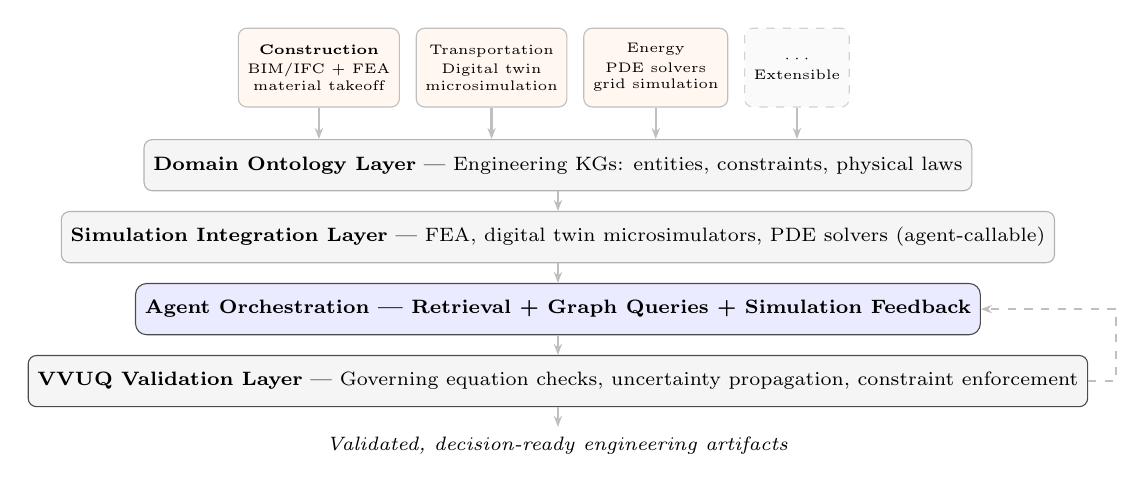
\begin{tikzpicture}[
        node distance=0.30cm and 0.20cm,
        layerbox/.style={rectangle, rounded corners=3pt, draw=gray!60, fill=gray!8, minimum width=7.8cm, minimum height=0.65cm, align=center, font=\scriptsize},
        dombox/.style={rectangle, rounded corners=3pt, draw=gray!50, fill=orange!6, minimum width=1.75cm, minimum height=1.0cm, align=center, font=\tiny},
        extbox/.style={rectangle, rounded corners=3pt, draw=gray!35, fill=gray!4, minimum width=1.05cm, minimum height=1.0cm, align=center, font=\tiny, dashed},
        agentbox/.style={rectangle, rounded corners=4pt, draw=black!70, fill=blue!8, minimum width=7.8cm, minimum height=0.65cm, align=center, font=\scriptsize\bfseries},
        arr/.style={-{Stealth[length=4pt]}, thick, gray!50},
    ]
        \node[dombox] (con) {\textbf{Construction}\\[1pt]BIM/IFC + FEA\\material takeoff};
        \node[dombox, right=0.20cm of con] (traf) {Transportation\\[1pt]Digital twin\\microsimulation};
        \node[dombox, right=0.20cm of traf] (energy) {Energy\\[1pt]PDE solvers\\grid simulation};
        \node[extbox, right=0.20cm of energy] (ext) {$\cdots$\\Extensible};

        \node[layerbox, below=0.40cm of $(con.south)!0.5!(ext.south)$] (onto) {\textbf{Domain Ontology Layer} --- Engineering KGs: entities, constraints, physical laws};

        \node[layerbox, below=0.25cm of onto] (sim) {\textbf{Simulation Integration Layer} --- FEA, digital twin microsimulators, PDE solvers (agent-callable)};

        \node[agentbox, below=0.25cm of sim] (agent) {Agent Orchestration --- Retrieval + Graph Queries + Simulation Feedback};

        \node[layerbox, below=0.25cm of agent, draw=black!70] (val) {\textbf{VVUQ Validation Layer} --- Governing equation checks, uncertainty propagation, constraint enforcement};

        \node[font=\scriptsize, below=0.25cm of val] (out) {\textit{Validated, decision-ready engineering artifacts}};

        \draw[arr] (con.south) -- (con.south |- onto.north);
        \draw[arr] (traf.south) -- (traf.south |- onto.north);
        \draw[arr] (energy.south) -- (energy.south |- onto.north);
        \draw[arr] (ext.south) -- (ext.south |- onto.north);
        \draw[arr] (onto) -- (sim);
        \draw[arr] (sim) -- (agent);
        \draw[arr] (agent) -- (val);
        \draw[arr] (val) -- (out);
        \draw[arr, dashed] (val.east) -- ++(0.35,0) |- (agent.east);
    \end{tikzpicture}
    }%
    \caption{\textbf{AKG-E Architecture.} Domain modules (Construction: primary; Transportation, Energy: extensions) plug into shared ontology, simulation, and VVUQ layers. The dashed feedback arrow represents iterative constraint-driven refinement.}
    \label{fig:framework}
    \vspace{-0.5em}
\end{figure}

The \textit{net-new contribution} that AKG-E adds beyond prior KG+agent systems is the explicit \textbf{agentic propose~$\to$~VVUQ~$\to$~feedback loop}: an agent emits a candidate engineering artifact, the VVUQ gate executes governing-equation residual checks, code-compliance lookups, and regulatory-constraint satisfiability tests with Monte Carlo-propagated uncertainty bounds, and returns a structured pass/fail decision that the agent must consume to refine the next iteration. The KG and the simulator are not new objects in isolation; the contribution is the typed, iterable control loop that couples them so that no artifact leaves the system without certified bounds. Unlike text-based critic loops or single-step retrieval-validity gates---which can flag inconsistency in prose but cannot certify physical or regulatory satisfaction---AKG-E's gate closes against \textit{quantitative simulation outputs} held to \textit{codified engineering standards}, enabling iterative validation at simulation-loop speed.

\section{Research Plan}

\subsection{Research Objectives}

This project pursues three objectives. \textbf{Objective~1 (Framework):} generalize the existing LVL VVUQ pipeline into the AKG-E framework---a typed, agent-callable propose~$\to$~VVUQ~$\to$~feedback loop coupling a domain knowledge graph, a simulation tool surface, and a governing-equation / code-compliance / constraint-satisfiability validation gate. \textbf{Objective~2 (Validation):} demonstrate AKG-E on two engineering domains (construction: BIM/IFC + FEA against AWC-NDS; transportation: digital-twin microsimulation against HCM2022) and measure the three-tier metrics---correctness, calibration, efficiency---against B0/B1/B2 baselines. \textbf{Objective~3 (Dissemination):} release the AKG-E framework, KG ontology templates, the simulator-tool interface specification, and the cross-domain benchmark as open source; publish peer-reviewed results in AI-for-engineering and agentic-AI venues.

\subsection{Methodology}

\textbf{Agent~$\leftrightarrow$~VVUQ-gate protocol.} The propose-VVUQ-feedback loop is implemented as a typed call/response: the agent emits an artifact specification (e.g., a header assembly with member sizes, materials, fasteners, and tributary-load assumptions) serialized to the domain ontology schema; the VVUQ gate ingests the artifact and runs three classes of checks: (i)~\textit{governing-equation residuals}---for the construction pilot, the Euler--Bernoulli relation $EI\,d^4w/dx^4 = q(x)$ is solved (analytically where available, numerically via FEniCS~\cite{Logg2012FEniCS} otherwise) and residuals on bending stress $\sigma=Mc/I$, shear $\tau=VQ/(Ib)$, and deflection $\delta$ are computed; (ii)~\textit{code-compliance lookups} against the ontology---AWC-NDS allowable-stress tables for the construction pilot, HCM2022 LOS thresholds for transportation, NERC-TPL contingency criteria for energy---returning a per-constraint pass/fail with the violated clause cited; and (iii)~\textit{regulatory-constraint satisfiability} via SMT-style queries over the KG to flag interactions among code provisions that any single lookup would miss. The gate returns a structured response: per-check pass/fail flags, the violated provisions, and 95\% confidence intervals on every scalar output. The agent consumes the response, locates the failing constraint, and either revises the artifact (e.g., increases header size, adjusts fastener schedule) or escalates to human-in-the-loop. The loop iterates until all checks pass or a tightened iteration budget is exhausted, at which point the best-so-far artifact is returned with its UQ envelope flagged.

\textbf{Uncertainty propagation.} Monte Carlo sampling is applied jointly over (a) simulator inputs---tributary widths, distributed loads, modulus of elasticity, demand profiles, grid contingency states---modeled as random variables with priors elicited from codified design tables and prior-art reliability literature, and (b) agent sampling temperature, so that the propagated 95\% CI captures both the simulator's epistemic uncertainty and the LLM's stochasticity. For each artifact, $N=1000$ MC samples is the default; convergence is tested against $N=10{,}000$ during verification, with all draws traced through the KG to preserve provenance.

\textbf{Construction-pilot specifics.} The pilot reuses three already-implemented modules from the construction-ai prototype: a BIM/IFC parser~\cite{Eastman2011BIM} that lifts wall, opening, and load-path entities into the KG; a typed FEA tool-call surface that wraps FEniCS solvers behind a stable agent-callable interface; and a refinement step that closes the loop by translating gate-emitted violations (e.g., ``deflection $0.42$~in exceeds $L/240=0.40$~in'') back into KG-conditioned prompts for the next iteration. The LVL VVUQ pipeline already operational in construction-ai supplies the methodology anchor and the closed-form verification baseline; AKG-E generalizes its Euler--Bernoulli + Monte Carlo pattern into the iterable propose-validate-refine protocol above.

\subsection{Evaluation Plan}

The evaluation enforces a three-tier metric framework that refines the abstract's constraint-violation reduction target into a more rigorous structure: correctness (the abstract's $>$50\% violation-reduction target preserved as the must-pass floor), calibration, and efficiency. \textbf{Correctness} is the non-negotiable floor: \textit{constraint-violation rate} measured against codified standards---AWC-NDS / IBC2021 (construction), HCM2022 LOS thresholds (transportation), NERC-TPL contingency criteria (energy, designed extension)---must approach zero on the benchmark and be statistically lower than every baseline. Agents that are fast and wrong are unfundable in safety-critical engineering. \textbf{Calibration}: the empirical coverage probability of the propagated 95\% CI must contain the ground truth in $\geq$95\% of benchmark tasks; calibration is validated against FEA reference designs (construction domain, via the LVL VVUQ pipeline outputs) and microsimulation reference outcomes (transportation domain, via the existing VTTI digital-twin proposal). \textbf{Efficiency} (headline contribution): wall-clock time-to-validated-decision per task is compared to the status-quo manufacturer-cycle baseline (weeks-to-months for construction VVUQ done by manufacturers); AKG-E targets minutes-to-hours per task at codified-standard correctness with calibrated UQ.

\textbf{Baselines (three-tier ablation):} \textbf{B0}~Claude alone (LLM-only; no retrieval, no validation loop); \textbf{B1}~Claude~+~graph-RAG over the curated domain KG (retrieval without the agentic VVUQ loop); \textbf{B2}~Claude~+~graph-RAG~+~agentic VVUQ loop (full AKG-E---this is the contribution). Each tier is run on the same benchmark, identical retrieval index, and identical prompt scaffold up to the loop boundary, so the marginal effect of the VVUQ loop is isolated.

\textbf{Benchmark suite.} The funded benchmark covers two domains, with a third designed in for future extension. \textit{Construction (funded)}: header sizing and material takeoff with AWC-NDS code-compliance checks; ground truth from the LVL VVUQ pipeline and AWC-NDS reference designs. \textit{Transportation (funded)}: signal-timing and digital-twin scenarios drawn from the existing VTTI VTSI proposal; ground truth from microsimulation outcomes and HCM LOS targets. \textit{Energy (designed extension)}: the three AKG-E layers apply to grid contingency analysis (NERC-TPL criteria) by swapping only the domain KG and PDE-solver interface; a proof-of-concept task is scheduled for Months~4--12 to demonstrate the domain-swap claim empirically. \textbf{Statistical analysis:} $n=5$ seeds minimum per (domain~$\times$~baseline) cell; 95\% bootstrap confidence intervals on all three metrics; significance threshold $p<0.05$ for headline claims. All three metrics are reported for every cell---no cherry-picking which metric to feature per condition.

\section{Timeline, Deliverables, and Risks}

The funded year begins \textbf{August 2026} and is structured as a 3-month aggressive build (M1--M3, Aug--Oct 2026) followed by 9 months of dissemination, robustness, scaling, and the energy-domain extension (M4--M12, Nov 2026--Jul 2027). Table~\ref{tab:gantt} maps the workstreams onto the calendar.

\begin{table*}[!ht]
\centering
\renewcommand{\arraystretch}{1.15}
\setlength{\tabcolsep}{4pt}
\caption{Project timeline. \textbf{M1--M3} is the aggressive build phase; \textbf{M4--M12} delivers dissemination, robustness, scaling, and the energy domain-swap proof-of-concept that demonstrates AKG-E's extensibility claim.}
\label{tab:gantt}
\footnotesize
\begin{tabular}{p{2.7in}|cccccccccccc}
\toprule
\textbf{Activity} & \multicolumn{12}{c}{\textbf{Month (Aug 2026 -- Jul 2027)}} \\
& M1 & M2 & M3 & M4 & M5 & M6 & M7 & M8 & M9 & M10 & M11 & M12 \\
\midrule
Framework: agentic propose$\to$VVUQ$\to$feedback loop & \gantt & \gantt & \gantt & & & & & & & & & \\
Construction pilot: LVL VVUQ generalization (BIM/IFC + FEA) & \gantt & \gantt & \gantt & & & & & & & & & \\
Transportation pilot: digital-twin microsim integration & & \gantt & \gantt & \gantt & & & & & & & & \\
Benchmark suite: B0 / B1 / B2 $\times$ 2 domains $\times$ $n{\geq}5$ seeds & & & \gantt & \gantt & \gantt & & & & & & & \\
Statistical analysis + first paper draft & & & & & \gantt & \gantt & & & & & & \\
Energy extension: NERC-TPL KG + PDE-solver interface (POC) & & & & & \gantt & \gantt & \gantt & \gantt & & & & \\
Robustness experiments (model swaps, prompt perturbations) & & & & & & & \gantt & \gantt & \gantt & \gantt & & \\
Scaling studies on AWS Bedrock & & & & & & & & \gantt & \gantt & \gantt & \gantt & \gantt \\
Publications + open-source release & & & & & & & & & & \gantt & \gantt & \gantt \\
\bottomrule
\end{tabular}
\end{table*}

\textit{Build phase rationale (M1--M3).} The construction-pilot anchor reuses the existing LVL VVUQ pipeline (BIM/IFC parser, FEniCS tool-call surface, Monte Carlo refinement), so M1 \textit{generalizes} existing code rather than green-fielding the framework; the transportation pilot lands per the existing VTTI digital-twin proposal across M2--M4; the cross-domain benchmark begins on construction and adds transportation as the second pilot stabilizes, with statistical analysis and the first paper draft completing in M5--M6.
\textit{Extension phase (M4--M12).} The energy domain-swap POC (NERC-TPL KG + PDE-solver interface) empirically validates the framework's extensibility claim across M5--M8 by swapping only the domain KG and simulator without modifying the shared ontology, simulation-integration, or VVUQ-validation layers. Robustness experiments stress-test model swaps and prompt perturbations; AWS Bedrock scaling studies establish the deployment surface; the final quarter delivers publications and the open-source release.
\textit{Deliverables:} (1)~the open-source AKG-E framework; (2)~domain-adaptable KG ontology templates and the typed FEA / digital-twin / PDE simulator-tool interface specification; (3)~the cross-domain benchmark with ground-truth datasets (construction + transportation funded, energy POC for the extensibility demonstration); (4)~peer-reviewed publications targeting AI-for-engineering and agentic-AI venues.

\textbf{Risks and Mitigation.} \textit{(a)~Agentic VVUQ loop slow to converge.} The propose-validate-refine loop may iterate beyond budget on edge cases. Mitigation: cap iterations at $K=10$ per artifact and accept best-so-far with explicit UQ caveats; this preserves correctness and calibration metrics while exposing efficiency as the variable under study. \textit{(b)~Code-compliance ontology completeness.} The AWC-NDS and HCM2022 corpora are large; if the curated KG ontology misses provisions, the gate may undercount violations. Mitigation: prioritize the highest-frequency provisions in the benchmark suite (header sizing for construction; uninterrupted-flow segments for transportation) and document ontology-coverage scope explicitly so reviewers can interpret reported violation rates against a stated provision boundary; coverage expands in Months~4--6 before publication. \textit{(c)~Benchmark ground-truth coverage thinner than expected.} If curating AWC-NDS reference designs or HCM-validated microsimulation scenarios takes longer than budgeted, mitigation is to ship a minimum-viable benchmark exercising B0/B1/B2 across a reduced task taxonomy in Month~3 and expand the suite in Months~4--6 before publication; the three-tier metrics remain reportable on the MVP, and the energy extension's KG-schema design proceeds in parallel rather than after.

\section{Team and Capabilities}

\textbf{Dr.~Kereshmeh Afsari (PI)} directs the ARCADE Lab at the Myers-Lawson School of Construction, with deep expertise in BIM, 3D visualization, and the construction-AI initiative that supplies AKG-E's primary domain testbed; she owns the ARCADE infrastructure (BIM/IFC datasets, simulation pipelines, AWS account) and the construction-industry partnerships that anchor the LVL pilot. \textbf{Dr.~Chris Brown (Co-PI)} in the Department of Computer Science at Virginia Tech contributes expertise in software engineering tooling and the empirical evaluation of AI-generated code, including the Brown--Cusati study of LLM behavior on software-engineering tasks that surfaced the verification weaknesses AKG-E sets out to close, and advises the student-research thread on agentic knowledge graphs. \textbf{Jason Cusati (Student Researcher)} brings the agentic-KG research-progression substrate that supplies AKG-E's orchestration layer, the VTTI Virginia Transportation Safety Index calculator (and its digital-twin extension proposal) that anchors the transportation domain, and direct VVUQ training under Dr.~Christopher Roy's graduate coursework (Oberkampf--Roy formulation~\cite{Oberkampf2010VVUQ}).

\textbf{Two Graduate Research Assistants full-time} during the 3-month build provide the engineering bandwidth. Three working prototypes ground the feasibility argument and align directly with the build plan: (1)~the LVL VVUQ pipeline (Euler--Bernoulli + Monte Carlo over BIM/IFC inputs) already operational in the construction-ai system, supplying the methodology anchor for Month~1's generalization step; (2)~the construction-ai KG + multi-agent material-takeoff web application, supplying the agent-orchestration substrate; and (3)~the existing VTTI transportation digital-twin proposal, supplying the Month~2 implementation target. ARCADE Lab provides BIM/IFC reference datasets, FEA simulation pipelines, and the AWS account that hosts the benchmark infrastructure.

\section{Intellectual Merit and Amazon Fit}

\textbf{Intellectual merit:} AKG-E contributes a principled VVUQ methodology for agentic AI outputs---a generalizable result that separates domain knowledge from shared orchestration and validation, and that is testable, falsifiable, and reusable across engineering disciplines. \textbf{Broader impact:} certified AI for safety-critical engineering---reducing hallucinated designs, enforcing code compliance, and enabling principled human-in-the-loop thresholds in workflows where errors carry legal and physical consequences. \textbf{Amazon fit:} AKG-E targets deployment via Amazon Bedrock Knowledge Bases~\cite{AWSBedrockHybridSearch2024}; the construction-logistics workflows around AWS-scale supply chains are the most direct downstream consumer; and the AWS-scale data pipelines the framework integrates with make AKG-E immediately relevant to Amazon's applied AI and construction-logistics roadmap.

\bibliographystyle{IEEEtran}
\bibliography{references}

\end{document}
